\begin{frame}[fragile]
  \frametitle{What is PNMR?}
  PNMR, or Pulsed Nuclear Magnetic Resonance, falls under the umbrella of MRI techniques that many of us are familiar with. 
  \begin{figure}
  \begin{center}
        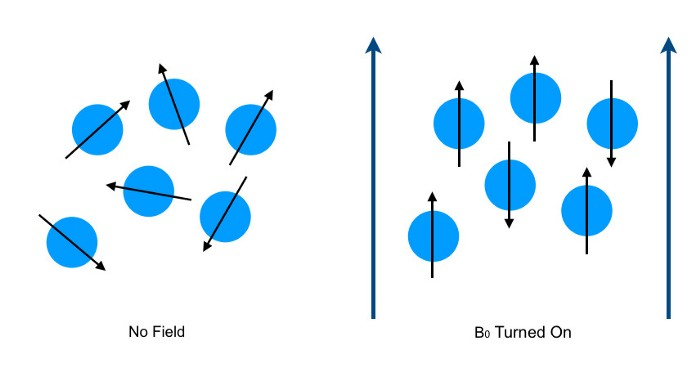
\includegraphics[height=5cm]{./images/polarization.jpeg}
\end{center}
\caption{Initial Polarization \cite{init_polar}}
\label{fig:relax}
\end{figure}
\end{frame}

\begin{frame}
  \frametitle{Relaxation Path}
  % a comment
  \begin{figure}[htbp!]
    \begin{center}
      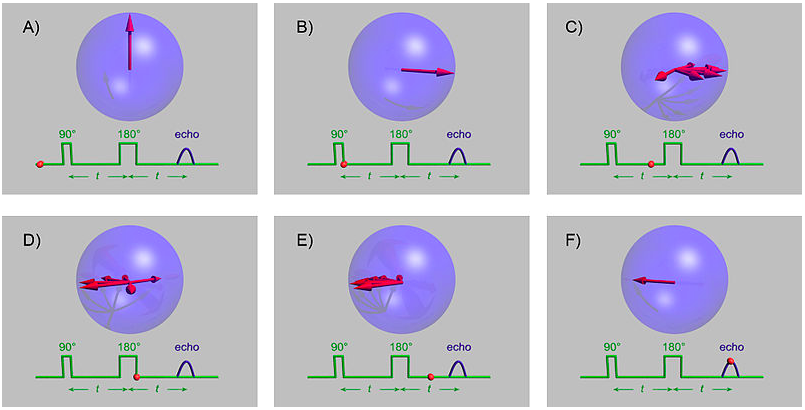
\includegraphics[height=5.2cm]{./images/figures/theory/relax.png}
    \end{center}
          \caption{General Relaxation Path \cite{spin_echo}}
    \label{fig:relax}
  \end{figure}
\end{frame}

\begin{frame}
  \frametitle{$90^{\circ}$ Pulses}
  % a comment
        \begin{center}
                \begin{figure}
                \begin{center}
                        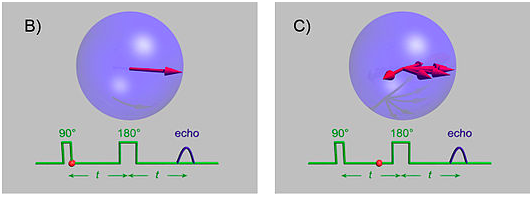
\includegraphics[width=\linewidth]{./images/Figures/theory/90deg.png}
                \end{center}
                \caption{Result of the $90^{\circ}$ Pulse \cite{spin_echo}}
                \label{fig:90_deg}
                \end{figure}
        \end{center}
\end{frame}

\begin{frame}
  \frametitle{$180^{\circ}$ Pulses}
  % a comment
        \begin{center}
                \begin{figure}
                \begin{center}
                        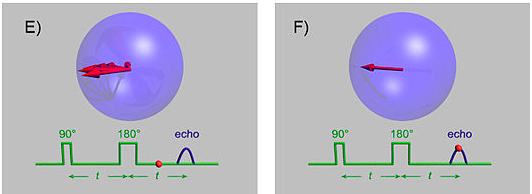
\includegraphics[width=\linewidth]{./images/Figures/theory/180deg.png}
                \end{center}
                \caption{Result of the $180^{\circ}$ Pulse \cite{spin_echo}}
                \label{fig:180_deg}
                \end{figure}
        \end{center}
\end{frame}
